% Figura do referencial: gráfico de cascata (waterfall) do exemplo hipotético da Seção de interpretabilidade local.
\begin{figure}[H]
    \centering
    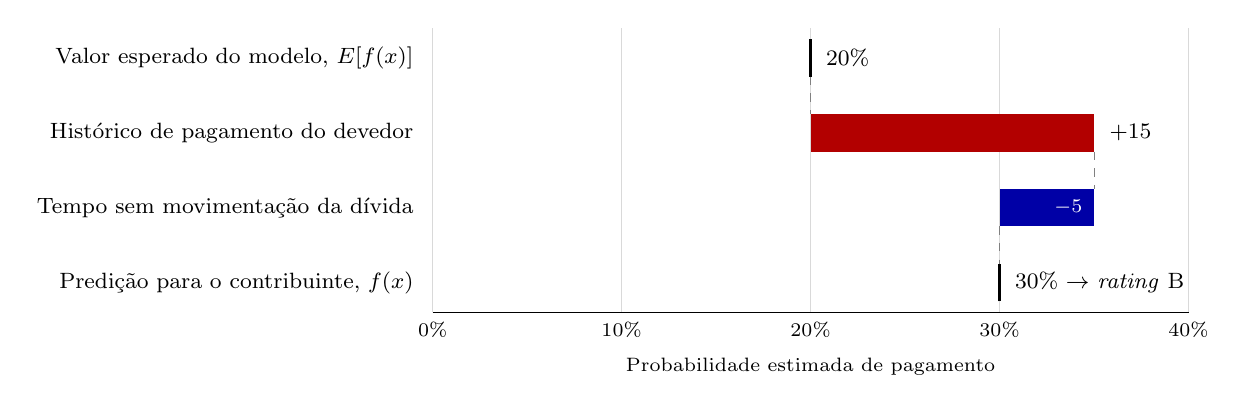
\begin{tikzpicture}[font=\footnotesize, x=0.24cm, y=0.95cm]
        % Eixo: probabilidade de pagamento, de 0% a 40%
        \foreach \v in {0,10,20,30,40} {
            \draw[gray!30] (\v,0.4) -- (\v,-3.4);
            \node[below, font=\scriptsize] at (\v,-3.4) {\v\%};
        }
        \draw (0,-3.4) -- (40,-3.4);
        \node[below=0.45cm, font=\scriptsize] at (20,-3.4) {Probabilidade estimada de pagamento};

        % Linha 1: valor esperado (ponto de partida)
        \node[left, align=right] at (-0.5,0) {Valor esperado do modelo, $E[f(x)]$};
        \draw[very thick] (20,-0.25) -- (20,0.25);
        \node[right] at (20.3,0) {20\%};

        % Linha 2: contribuição positiva
        \node[left, align=right] at (-0.5,-1) {Histórico de pagamento do devedor};
        \fill[red!70!black] (20,-1.25) rectangle (35,-0.75);
        \node[right] at (35.3,-1) {$+15$};
        \draw[dashed, gray] (20,-0.25) -- (20,-0.75);

        % Linha 3: contribuição negativa
        \node[left, align=right] at (-0.5,-2) {Tempo sem movimentação da dívida};
        \fill[blue!65!black] (30,-2.25) rectangle (35,-1.75);
        \node[left, text=white, font=\scriptsize\bfseries] at (34.9,-2) {$-5$};
        \draw[dashed, gray] (35,-1.25) -- (35,-1.75);

        % Linha 4: predição final
        \node[left, align=right] at (-0.5,-3) {Predição para o contribuinte, $f(x)$};
        \draw[very thick] (30,-3.25) -- (30,-2.75);
        \draw[dashed, gray] (30,-2.25) -- (30,-2.75);
        \node[right] at (30.3,-3) {30\% $\rightarrow$ \textit{rating} B};
    \end{tikzpicture}
    \caption[Decomposição de uma predição individual em um gráfico de cascata do SHAP]{Decomposição de uma predição individual em um gráfico de cascata (\textit{waterfall plot}) do SHAP, com o exemplo hipotético descrito no texto. A leitura é feita de cima para baixo: o ponto de partida é a probabilidade média estimada pelo modelo (20\%); cada barra soma a contribuição de uma variável, em vermelho quando aumenta a probabilidade de pagamento e em azul quando a reduz; o resultado é a predição para o contribuinte (30\%), que corresponde ao \textit{rating} B. A soma das contribuições é exatamente a diferença entre a predição e a média ($+15 - 5 = +10$ pontos), propriedade que permite atribuir a cada variável uma parcela exata da decisão.}
    \label{fig:shap_waterfall}
\end{figure}
